\documentclass[1p]{elsarticle_modified}
%\bibliographystyle{elsarticle-num}

%\usepackage[colorlinks]{hyperref}
%\usepackage{abbrmath_seonhwa} %\Abb, \Ascr, \Acal ,\Abf, \Afrak
\usepackage{amsfonts}
\usepackage{amssymb}
\usepackage{amsmath}
\usepackage{amsthm}
\usepackage{scalefnt}
\usepackage{amsbsy}
\usepackage{kotex}
\usepackage{caption}
\usepackage{subfig}
\usepackage{color}
\usepackage{graphicx}
\usepackage{xcolor} %% white, black, red, green, blue, cyan, magenta, yellow
\usepackage{float}
\usepackage{setspace}
\usepackage{hyperref}

\usepackage{tikz}
\usetikzlibrary{arrows}

\usepackage{multirow}
\usepackage{array} % fixed length table
\usepackage{hhline}

%%%%%%%%%%%%%%%%%%%%%
\makeatletter
\renewcommand*\env@matrix[1][\arraystretch]{%
	\edef\arraystretch{#1}%
	\hskip -\arraycolsep
	\let\@ifnextchar\new@ifnextchar
	\array{*\c@MaxMatrixCols c}}
\makeatother %https://tex.stackexchange.com/questions/14071/how-can-i-increase-the-line-spacing-in-a-matrix
%%%%%%%%%%%%%%%

\usepackage[normalem]{ulem}

\newcommand{\msout}[1]{\ifmmode\text{\sout{\ensuremath{#1}}}\else\sout{#1}\fi}
%SOURCE: \msout is \stkout macro in https://tex.stackexchange.com/questions/20609/strikeout-in-math-mode

\newcommand{\cancel}[1]{
	\ifmmode
	{\color{red}\msout{#1}}
	\else
	{\color{red}\sout{#1}}
	\fi
}

\newcommand{\add}[1]{
	{\color{blue}\uwave{#1}}
}

\newcommand{\replace}[2]{
	\ifmmode
	{\color{red}\msout{#1}}{\color{blue}\uwave{#2}}
	\else
	{\color{red}\sout{#1}}{\color{blue}\uwave{#2}}
	\fi
}

\newcommand{\Sol}{\mathcal{S}} %segment
\newcommand{\D}{D} %diagram
\newcommand{\A}{\mathcal{A}} %arc


%%%%%%%%%%%%%%%%%%%%%%%%%%%%%5 test

\def\sl{\operatorname{\textup{SL}}(2,\Cbb)}
\def\psl{\operatorname{\textup{PSL}}(2,\Cbb)}
\def\quan{\mkern 1mu \triangleright \mkern 1mu}

\theoremstyle{definition}
\newtheorem{thm}{Theorem}[section]
\newtheorem{prop}[thm]{Proposition}
\newtheorem{lem}[thm]{Lemma}
\newtheorem{ques}[thm]{Question}
\newtheorem{cor}[thm]{Corollary}
\newtheorem{defn}[thm]{Definition}
\newtheorem{exam}[thm]{Example}
\newtheorem{rmk}[thm]{Remark}
\newtheorem{alg}[thm]{Algorithm}

\newcommand{\I}{\sqrt{-1}}
\begin{document}

%\begin{frontmatter}
%
%\title{Boundary parabolic representations of knots up to 8 crossings}
%
%%% Group authors per affiliation:
%\author{Yunhi Cho} 
%\address{Department of Mathematics, University of Seoul, Seoul, Korea}
%\ead{yhcho@uos.ac.kr}
%
%
%\author{Seonhwa Kim} %\fnref{s_kim}}
%\address{Center for Geometry and Physics, Institute for Basic Science, Pohang, 37673, Korea}
%\ead{ryeona17@ibs.re.kr}
%
%\author{Hyuk Kim}
%\address{Department of Mathematical Sciences, Seoul National University, Seoul 08826, Korea}
%\ead{hyukkim@snu.ac.kr}
%
%\author{Seokbeom Yoon}
%\address{Department of Mathematical Sciences, Seoul National University, Seoul, 08826,  Korea}
%\ead{sbyoon15@snu.ac.kr}
%
%\begin{abstract}
%We find all boundary parabolic representation of knots up to 8 crossings.
%
%\end{abstract}
%\begin{keyword}
%    \MSC[2010] 57M25 
%\end{keyword}
%
%\end{frontmatter}

%\linenumbers
%\tableofcontents
%
\newcommand\colored[1]{\textcolor{white}{\rule[-0.35ex]{0.8em}{1.4ex}}\kern-0.8em\color{red} #1}%
%\newcommand\colored[1]{\textcolor{white}{ #1}\kern-2.17ex	\textcolor{white}{ #1}\kern-1.81ex	\textcolor{white}{ #1}\kern-2.15ex\color{red}#1	}

{\Large $\underline{12a_{1198}~(K12a_{1198})}$}

\setlength{\tabcolsep}{10pt}
\renewcommand{\arraystretch}{1.6}
\vspace{1cm}\begin{tabular}{m{100pt}>{\centering\arraybackslash}m{274pt}}
\multirow{5}{120pt}{
	\centering
	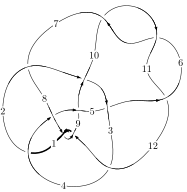
\includegraphics[width=112pt]{../../../GIT/diagram.site/Diagrams/png/1999_12a_1198.png}\\
\ \ \ A knot diagram\footnotemark}&
\allowdisplaybreaks
\textbf{Linearized knot diagam} \\
\cline{2-2}
 &
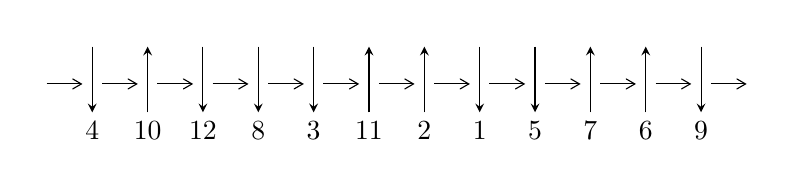
\begin{tikzpicture}[x=20pt, y=17pt]
	% nodes
	\node (C0) at (0, 0) {};
	\node (C1) at (1, 0) {};
	\node (C1U) at (1, +1) {};
	\node (C1D) at (1, -1) {4};

	\node (C2) at (2, 0) {};
	\node (C2U) at (2, +1) {};
	\node (C2D) at (2, -1) {10};

	\node (C3) at (3, 0) {};
	\node (C3U) at (3, +1) {};
	\node (C3D) at (3, -1) {12};

	\node (C4) at (4, 0) {};
	\node (C4U) at (4, +1) {};
	\node (C4D) at (4, -1) {8};

	\node (C5) at (5, 0) {};
	\node (C5U) at (5, +1) {};
	\node (C5D) at (5, -1) {3};

	\node (C6) at (6, 0) {};
	\node (C6U) at (6, +1) {};
	\node (C6D) at (6, -1) {11};

	\node (C7) at (7, 0) {};
	\node (C7U) at (7, +1) {};
	\node (C7D) at (7, -1) {2};

	\node (C8) at (8, 0) {};
	\node (C8U) at (8, +1) {};
	\node (C8D) at (8, -1) {1};

	\node (C9) at (9, 0) {};
	\node (C9U) at (9, +1) {};
	\node (C9D) at (9, -1) {5};

	\node (C10) at (10, 0) {};
	\node (C10U) at (10, +1) {};
	\node (C10D) at (10, -1) {7};

	\node (C11) at (11, 0) {};
	\node (C11U) at (11, +1) {};
	\node (C11D) at (11, -1) {6};

	\node (C12) at (12, 0) {};
	\node (C12U) at (12, +1) {};
	\node (C12D) at (12, -1) {9};
	\node (C13) at (13, 0) {};

	% arrows
	\draw[->,>={angle 60}]
	(C0) edge (C1) (C1) edge (C2) (C2) edge (C3) (C3) edge (C4) (C4) edge (C5) (C5) edge (C6) (C6) edge (C7) (C7) edge (C8) (C8) edge (C9) (C9) edge (C10) (C10) edge (C11) (C11) edge (C12) (C12) edge (C13) ;	\draw[->,>=stealth]
	(C1U) edge (C1D) (C2D) edge (C2U) (C3U) edge (C3D) (C4U) edge (C4D) (C5U) edge (C5D) (C6D) edge (C6U) (C7D) edge (C7U) (C8U) edge (C8D) (C9U) edge (C9D) (C10D) edge (C10U) (C11D) edge (C11U) (C12U) edge (C12D) ;
	\end{tikzpicture} \\
\hhline{~~} \\& 
\textbf{Solving Sequence} \\ \cline{2-2} 
 &
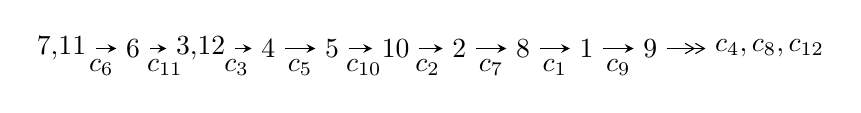
\begin{tikzpicture}[x=23pt, y=7pt]
	% node
	\node (A0) at (-1/8, 0) {7,11};
	\node (A1) at (1, 0) {6};
	\node (A2) at (33/16, 0) {3,12};
	\node (A3) at (25/8, 0) {4};
	\node (A4) at (33/8, 0) {5};
	\node (A5) at (41/8, 0) {10};
	\node (A6) at (49/8, 0) {2};
	\node (A7) at (57/8, 0) {8};
	\node (A8) at (65/8, 0) {1};
	\node (A9) at (73/8, 0) {9};
	\node (C1) at (1/2, -1) {$c_{6}$};
	\node (C2) at (3/2, -1) {$c_{11}$};
	\node (C3) at (21/8, -1) {$c_{3}$};
	\node (C4) at (29/8, -1) {$c_{5}$};
	\node (C5) at (37/8, -1) {$c_{10}$};
	\node (C6) at (45/8, -1) {$c_{2}$};
	\node (C7) at (53/8, -1) {$c_{7}$};
	\node (C8) at (61/8, -1) {$c_{1}$};
	\node (C9) at (69/8, -1) {$c_{9}$};
	\node (A10) at (11, 0) {$c_{4},c_{8},c_{12}$};

	% edge
	\draw[->,>=stealth]	
	(A0) edge (A1) (A1) edge (A2) (A2) edge (A3) (A3) edge (A4) (A4) edge (A5) (A5) edge (A6) (A6) edge (A7) (A7) edge (A8) (A8) edge (A9) ;
	\draw[->>,>={angle 60}]	
	(A9) edge (A10);
\end{tikzpicture} \\ 

\end{tabular} \\

\footnotetext{
The image of knot diagram is generated by the software ``\textbf{Draw programme}" developed by Andrew Bartholomew(\url{http://www.layer8.co.uk/maths/draw/index.htm\#Running-draw}), where we modified some parts for our purpose(\url{https://github.com/CATsTAILs/LinksPainter}).
}\phantom \\ \newline 
\centering \textbf{Ideals for irreducible components\footnotemark of $X_{\text{par}}$} 
 
\begin{align*}
I^u_{1}&=\langle 
4.66736\times10^{443} u^{144}-4.79119\times10^{444} u^{143}+\cdots+1.30096\times10^{445} b-6.96891\times10^{445},\\
\phantom{I^u_{1}}&\phantom{= \langle  }7.40283\times10^{445} u^{144}-2.14361\times10^{446} u^{143}+\cdots+1.30096\times10^{445} a+1.08136\times10^{447},\\
\phantom{I^u_{1}}&\phantom{= \langle  }u^{145}-3 u^{144}+\cdots+30 u+1\rangle \\
I^u_{2}&=\langle 
20500548319041 u^{33}-275174690960662 u^{32}+\cdots+673397680793441 b-65230091246849,\\
\phantom{I^u_{2}}&\phantom{= \langle  }528075704142869 u^{33}+297599063074788 u^{32}+\cdots+673397680793441 a+2532338124697314,\\
\phantom{I^u_{2}}&\phantom{= \langle  }u^{34}+18 u^{32}+\cdots+2 u+1\rangle \\
\\
\end{align*}
\raggedright * 2 irreducible components of $\dim_{\mathbb{C}}=0$, with total 179 representations.\\
\footnotetext{All coefficients of polynomials are rational numbers. But the coefficients are sometimes approximated in decimal forms when there is not enough margin.}
\newpage
\renewcommand{\arraystretch}{1}
\centering \section*{I. $I^u_{1}= \langle 4.67\times10^{443} u^{144}-4.79\times10^{444} u^{143}+\cdots+1.30\times10^{445} b-6.97\times10^{445},\;7.40\times10^{445} u^{144}-2.14\times10^{446} u^{143}+\cdots+1.30\times10^{445} a+1.08\times10^{447},\;u^{145}-3 u^{144}+\cdots+30 u+1 \rangle$}
\flushleft \textbf{(i) Arc colorings}\\
\begin{tabular}{m{7pt} m{180pt} m{7pt} m{180pt} }
\flushright $a_{7}=$&$\begin{pmatrix}1\\0\end{pmatrix}$ \\
\flushright $a_{11}=$&$\begin{pmatrix}0\\u\end{pmatrix}$ \\
\flushright $a_{6}=$&$\begin{pmatrix}1\\u^2\end{pmatrix}$ \\
\flushright $a_{3}=$&$\begin{pmatrix}-5.69028 u^{144}+16.4771 u^{143}+\cdots-1416.60 u-83.1200\\-0.0358763 u^{144}+0.368281 u^{143}+\cdots+115.079 u+5.35674\end{pmatrix}$ \\
\flushright $a_{12}=$&$\begin{pmatrix}u\\u^3+u\end{pmatrix}$ \\
\flushright $a_{4}=$&$\begin{pmatrix}-5.48647 u^{144}+15.6291 u^{143}+\cdots-1397.04 u-82.6558\\0.164018 u^{144}+0.220810 u^{143}+\cdots+141.533 u+6.05755\end{pmatrix}$ \\
\flushright $a_{5}=$&$\begin{pmatrix}1.97186 u^{144}-6.26110 u^{143}+\cdots+519.259 u+16.7480\\1.02742 u^{144}-2.88351 u^{143}+\cdots+105.297 u+5.45072\end{pmatrix}$ \\
\flushright $a_{10}=$&$\begin{pmatrix}- u\\u\end{pmatrix}$ \\
\flushright $a_{2}=$&$\begin{pmatrix}-5.94131 u^{144}+17.0043 u^{143}+\cdots-1432.32 u-83.4530\\0.215160 u^{144}-0.158920 u^{143}+\cdots+130.797 u+5.68982\end{pmatrix}$ \\
\flushright $a_{8}=$&$\begin{pmatrix}2.01176 u^{144}-6.54341 u^{143}+\cdots+128.662 u-4.11881\\0.344088 u^{144}-1.16477 u^{143}+\cdots+140.826 u+6.88706\end{pmatrix}$ \\
\flushright $a_{1}=$&$\begin{pmatrix}-3.88338 u^{144}+11.9704 u^{143}+\cdots-1279.86 u-85.6891\\-0.158624 u^{144}+0.126640 u^{143}+\cdots+80.8831 u+4.76537\end{pmatrix}$ \\
\flushright $a_{9}=$&$\begin{pmatrix}5.50348 u^{144}-17.0024 u^{143}+\cdots+1340.19 u+68.7005\\0.135896 u^{144}-0.505632 u^{143}+\cdots-7.74655 u+0.862548\end{pmatrix}$\\&\end{tabular}
\flushleft \textbf{(ii) Obstruction class $= -1$}\\~\\
\flushleft \textbf{(iii) Cusp Shapes $= -0.0387298 u^{144}+1.57838 u^{143}+\cdots+204.001 u+8.73476$}\\~\\
\newpage\renewcommand{\arraystretch}{1}
\flushleft \textbf{(iv) u-Polynomials at the component}\newline \\
\begin{tabular}{m{50pt}|m{274pt}}
Crossings & \hspace{64pt}u-Polynomials at each crossing \\
\hline $$\begin{aligned}c_{1}\end{aligned}$$&$\begin{aligned}
&u^{145}+6 u^{144}+\cdots-16 u+1
\end{aligned}$\\
\hline $$\begin{aligned}c_{2}\end{aligned}$$&$\begin{aligned}
&u^{145}+4 u^{144}+\cdots+185515060 u+38279399
\end{aligned}$\\
\hline $$\begin{aligned}c_{3}\end{aligned}$$&$\begin{aligned}
&u^{145}-35 u^{143}+\cdots-85631889 u+14144791
\end{aligned}$\\
\hline $$\begin{aligned}c_{4}\end{aligned}$$&$\begin{aligned}
&u^{145}+u^{144}+\cdots+2 u+1
\end{aligned}$\\
\hline $$\begin{aligned}c_{5}\end{aligned}$$&$\begin{aligned}
&u^{145}+12 u^{144}+\cdots-13174228 u+7328689
\end{aligned}$\\
\hline $$\begin{aligned}c_{6},c_{10},c_{11}\end{aligned}$$&$\begin{aligned}
&u^{145}-3 u^{144}+\cdots+30 u+1
\end{aligned}$\\
\hline $$\begin{aligned}c_{7}\end{aligned}$$&$\begin{aligned}
&u^{145}-2 u^{144}+\cdots+14370450736 u+2642976587
\end{aligned}$\\
\hline $$\begin{aligned}c_{8},c_{12}\end{aligned}$$&$\begin{aligned}
&u^{145}+49 u^{143}+\cdots+1759 u+541
\end{aligned}$\\
\hline $$\begin{aligned}c_{9}\end{aligned}$$&$\begin{aligned}
&u^{145}- u^{144}+\cdots+962205 u+328951
\end{aligned}$\\
\hline
\end{tabular}\\~\\
\newpage\renewcommand{\arraystretch}{1}
\flushleft \textbf{(v) Riley Polynomials at the component}\newline \\
\begin{tabular}{m{50pt}|m{274pt}}
Crossings & \hspace{64pt}Riley Polynomials at each crossing \\
\hline $$\begin{aligned}c_{1}\end{aligned}$$&$\begin{aligned}
&y^{145}-16 y^{144}+\cdots-758 y-1
\end{aligned}$\\
\hline $$\begin{aligned}c_{2}\end{aligned}$$&$\begin{aligned}
&y^{145}+64 y^{144}+\cdots-46211062606405672 y-1465312387801201
\end{aligned}$\\
\hline $$\begin{aligned}c_{3}\end{aligned}$$&$\begin{aligned}
&y^{145}-70 y^{144}+\cdots+9065639520733613 y-200075112433681
\end{aligned}$\\
\hline $$\begin{aligned}c_{4}\end{aligned}$$&$\begin{aligned}
&y^{145}+y^{144}+\cdots-30 y-1
\end{aligned}$\\
\hline $$\begin{aligned}c_{5}\end{aligned}$$&$\begin{aligned}
&y^{145}-46 y^{144}+\cdots+2078737869821982 y-53709682458721
\end{aligned}$\\
\hline $$\begin{aligned}c_{6},c_{10},c_{11}\end{aligned}$$&$\begin{aligned}
&y^{145}+151 y^{144}+\cdots+224 y-1
\end{aligned}$\\
\hline $$\begin{aligned}c_{7}\end{aligned}$$&$\begin{aligned}
&y^{145}+92 y^{144}+\cdots-3.02\times10^{20} y-6.99\times10^{18}
\end{aligned}$\\
\hline $$\begin{aligned}c_{8},c_{12}\end{aligned}$$&$\begin{aligned}
&y^{145}+98 y^{144}+\cdots-20435091 y-292681
\end{aligned}$\\
\hline $$\begin{aligned}c_{9}\end{aligned}$$&$\begin{aligned}
&y^{145}-15 y^{144}+\cdots+1990900220177 y-108208760401
\end{aligned}$\\
\hline
\end{tabular}\\~\\
\newpage\flushleft \textbf{(vi) Complex Volumes and Cusp Shapes}
$$\begin{array}{c|c|c}  
\text{Solutions to }I^u_{1}& \I (\text{vol} + \sqrt{-1}CS) & \text{Cusp shape}\\
 \hline 
\begin{aligned}
u &= \phantom{-}0.556225 + 0.825178 I \\
a &= -0.642250 - 0.113886 I \\
b &= -0.549441 + 0.390152 I\end{aligned}
 & -0.98641 + 5.89965 I & \phantom{-0.000000 } 0 \\ \hline\begin{aligned}
u &= \phantom{-}0.556225 - 0.825178 I \\
a &= -0.642250 + 0.113886 I \\
b &= -0.549441 - 0.390152 I\end{aligned}
 & -0.98641 - 5.89965 I & \phantom{-0.000000 } 0 \\ \hline\begin{aligned}
u &= \phantom{-}0.624539 + 0.774639 I \\
a &= \phantom{-}0.650404 - 0.195995 I \\
b &= \phantom{-}0.296229 + 0.396389 I\end{aligned}
 & \phantom{-}1.22895 + 2.67342 I & \phantom{-0.000000 } 0 \\ \hline\begin{aligned}
u &= \phantom{-}0.624539 - 0.774639 I \\
a &= \phantom{-}0.650404 + 0.195995 I \\
b &= \phantom{-}0.296229 - 0.396389 I\end{aligned}
 & \phantom{-}1.22895 - 2.67342 I & \phantom{-0.000000 } 0 \\ \hline\begin{aligned}
u &= -0.461064 + 0.896003 I \\
a &= -0.328974 - 0.451183 I \\
b &= -0.038803 - 0.414851 I\end{aligned}
 & \phantom{-}3.99268 - 5.21091 I & \phantom{-0.000000 } 0 \\ \hline\begin{aligned}
u &= -0.461064 - 0.896003 I \\
a &= -0.328974 + 0.451183 I \\
b &= -0.038803 + 0.414851 I\end{aligned}
 & \phantom{-}3.99268 + 5.21091 I & \phantom{-0.000000 } 0 \\ \hline\begin{aligned}
u &= -0.814275 + 0.598530 I \\
a &= \phantom{-}0.531502 - 0.489949 I \\
b &= \phantom{-}0.801664 + 0.014554 I\end{aligned}
 & -4.83166 - 9.34281 I & \phantom{-0.000000 } 0 \\ \hline\begin{aligned}
u &= -0.814275 - 0.598530 I \\
a &= \phantom{-}0.531502 + 0.489949 I \\
b &= \phantom{-}0.801664 - 0.014554 I\end{aligned}
 & -4.83166 + 9.34281 I & \phantom{-0.000000 } 0 \\ \hline\begin{aligned}
u &= \phantom{-}0.268368 + 0.984195 I \\
a &= \phantom{-}0.239016 - 0.542346 I \\
b &= -0.617928 + 0.932521 I\end{aligned}
 & -1.03551 + 1.06476 I & \phantom{-0.000000 } 0 \\ \hline\begin{aligned}
u &= \phantom{-}0.268368 - 0.984195 I \\
a &= \phantom{-}0.239016 + 0.542346 I \\
b &= -0.617928 - 0.932521 I\end{aligned}
 & -1.03551 - 1.06476 I & \phantom{-0.000000 } 0\\
 \hline 
 \end{array}$$\newpage$$\begin{array}{c|c|c}  
\text{Solutions to }I^u_{1}& \I (\text{vol} + \sqrt{-1}CS) & \text{Cusp shape}\\
 \hline 
\begin{aligned}
u &= \phantom{-}0.831486 + 0.608016 I \\
a &= \phantom{-}0.567344 + 0.572549 I \\
b &= \phantom{-}0.750347 - 0.119663 I\end{aligned}
 & -0.9751 + 15.4421 I & \phantom{-0.000000 } 0 \\ \hline\begin{aligned}
u &= \phantom{-}0.831486 - 0.608016 I \\
a &= \phantom{-}0.567344 - 0.572549 I \\
b &= \phantom{-}0.750347 + 0.119663 I\end{aligned}
 & -0.9751 - 15.4421 I & \phantom{-0.000000 } 0 \\ \hline\begin{aligned}
u &= \phantom{-}0.314618 + 0.987524 I \\
a &= \phantom{-}0.440419 + 0.325660 I \\
b &= -1.07228 - 1.17355 I\end{aligned}
 & \phantom{-}0.00642 - 3.18413 I & \phantom{-0.000000 } 0 \\ \hline\begin{aligned}
u &= \phantom{-}0.314618 - 0.987524 I \\
a &= \phantom{-}0.440419 - 0.325660 I \\
b &= -1.07228 + 1.17355 I\end{aligned}
 & \phantom{-}0.00642 + 3.18413 I & \phantom{-0.000000 } 0 \\ \hline\begin{aligned}
u &= \phantom{-}0.829458 + 0.625826 I \\
a &= -0.256361 - 0.647722 I \\
b &= -0.572982 + 0.100892 I\end{aligned}
 & -2.75410 + 3.14936 I & \phantom{-0.000000 } 0 \\ \hline\begin{aligned}
u &= \phantom{-}0.829458 - 0.625826 I \\
a &= -0.256361 + 0.647722 I \\
b &= -0.572982 - 0.100892 I\end{aligned}
 & -2.75410 - 3.14936 I & \phantom{-0.000000 } 0 \\ \hline\begin{aligned}
u &= -0.880427 + 0.572298 I \\
a &= -0.049833 - 0.547892 I \\
b &= \phantom{-}0.323661 - 0.448848 I\end{aligned}
 & -4.66504 + 3.72932 I & \phantom{-0.000000 } 0 \\ \hline\begin{aligned}
u &= -0.880427 - 0.572298 I \\
a &= -0.049833 + 0.547892 I \\
b &= \phantom{-}0.323661 + 0.448848 I\end{aligned}
 & -4.66504 - 3.72932 I & \phantom{-0.000000 } 0 \\ \hline\begin{aligned}
u &= \phantom{-}0.845795 + 0.633543 I \\
a &= \phantom{-}0.564688 + 0.294872 I \\
b &= \phantom{-}0.587663 + 0.436303 I\end{aligned}
 & \phantom{-}1.05971 + 2.93819 I & \phantom{-0.000000 } 0 \\ \hline\begin{aligned}
u &= \phantom{-}0.845795 - 0.633543 I \\
a &= \phantom{-}0.564688 - 0.294872 I \\
b &= \phantom{-}0.587663 - 0.436303 I\end{aligned}
 & \phantom{-}1.05971 - 2.93819 I & \phantom{-0.000000 } 0\\
 \hline 
 \end{array}$$\newpage$$\begin{array}{c|c|c}  
\text{Solutions to }I^u_{1}& \I (\text{vol} + \sqrt{-1}CS) & \text{Cusp shape}\\
 \hline 
\begin{aligned}
u &= \phantom{-}0.881992 + 0.588045 I \\
a &= \phantom{-}0.054193 - 0.456185 I \\
b &= -0.576587 - 0.134071 I\end{aligned}
 & -2.57032 + 2.58753 I & \phantom{-0.000000 } 0 \\ \hline\begin{aligned}
u &= \phantom{-}0.881992 - 0.588045 I \\
a &= \phantom{-}0.054193 + 0.456185 I \\
b &= -0.576587 + 0.134071 I\end{aligned}
 & -2.57032 - 2.58753 I & \phantom{-0.000000 } 0 \\ \hline\begin{aligned}
u &= \phantom{-}0.301316 + 0.886369 I \\
a &= \phantom{-}0.182491 + 0.204939 I \\
b &= -0.214326 + 0.398617 I\end{aligned}
 & -0.58432 + 1.86220 I & \phantom{-0.000000 } 0 \\ \hline\begin{aligned}
u &= \phantom{-}0.301316 - 0.886369 I \\
a &= \phantom{-}0.182491 - 0.204939 I \\
b &= -0.214326 - 0.398617 I\end{aligned}
 & -0.58432 - 1.86220 I & \phantom{-0.000000 } 0 \\ \hline\begin{aligned}
u &= -0.782451 + 0.502344 I \\
a &= -0.567424 + 1.000280 I \\
b &= -0.540958 - 0.208296 I\end{aligned}
 & -1.99261 - 6.01306 I & \phantom{-0.000000 } 0 \\ \hline\begin{aligned}
u &= -0.782451 - 0.502344 I \\
a &= -0.567424 - 1.000280 I \\
b &= -0.540958 + 0.208296 I\end{aligned}
 & -1.99261 + 6.01306 I & \phantom{-0.000000 } 0 \\ \hline\begin{aligned}
u &= \phantom{-}0.919012 + 0.570141 I \\
a &= -0.207431 + 0.457950 I \\
b &= \phantom{-}0.371977 + 0.477396 I\end{aligned}
 & -0.76501 - 9.68728 I & \phantom{-0.000000 } 0 \\ \hline\begin{aligned}
u &= \phantom{-}0.919012 - 0.570141 I \\
a &= -0.207431 - 0.457950 I \\
b &= \phantom{-}0.371977 - 0.477396 I\end{aligned}
 & -0.76501 + 9.68728 I & \phantom{-0.000000 } 0 \\ \hline\begin{aligned}
u &= -0.370483 + 0.808138 I \\
a &= \phantom{-}0.214317 - 1.287740 I \\
b &= -0.121966 - 0.078133 I\end{aligned}
 & \phantom{-}1.27250 + 4.48458 I & \phantom{-0.000000 } 0 \\ \hline\begin{aligned}
u &= -0.370483 - 0.808138 I \\
a &= \phantom{-}0.214317 + 1.287740 I \\
b &= -0.121966 + 0.078133 I\end{aligned}
 & \phantom{-}1.27250 - 4.48458 I & \phantom{-0.000000 } 0\\
 \hline 
 \end{array}$$\newpage$$\begin{array}{c|c|c}  
\text{Solutions to }I^u_{1}& \I (\text{vol} + \sqrt{-1}CS) & \text{Cusp shape}\\
 \hline 
\begin{aligned}
u &= -0.402766 + 0.783717 I \\
a &= \phantom{-}0.012063 + 0.733731 I \\
b &= -0.423670 - 1.059380 I\end{aligned}
 & -0.65449 - 2.56138 I & \phantom{-0.000000 } 0 \\ \hline\begin{aligned}
u &= -0.402766 - 0.783717 I \\
a &= \phantom{-}0.012063 - 0.733731 I \\
b &= -0.423670 + 1.059380 I\end{aligned}
 & -0.65449 + 2.56138 I & \phantom{-0.000000 } 0 \\ \hline\begin{aligned}
u &= \phantom{-}0.785549 + 0.331316 I \\
a &= \phantom{-}0.209417 - 0.240366 I \\
b &= -0.109209 + 0.642695 I\end{aligned}
 & \phantom{-}2.34000 + 2.19166 I & \phantom{-0.000000 } 0 \\ \hline\begin{aligned}
u &= \phantom{-}0.785549 - 0.331316 I \\
a &= \phantom{-}0.209417 + 0.240366 I \\
b &= -0.109209 - 0.642695 I\end{aligned}
 & \phantom{-}2.34000 - 2.19166 I & \phantom{-0.000000 } 0 \\ \hline\begin{aligned}
u &= -0.659761 + 0.535821 I \\
a &= \phantom{-}0.278189 + 0.370634 I \\
b &= -0.712055 + 0.496101 I\end{aligned}
 & -2.29633 + 1.12360 I & \phantom{-0.000000 } 0 \\ \hline\begin{aligned}
u &= -0.659761 - 0.535821 I \\
a &= \phantom{-}0.278189 - 0.370634 I \\
b &= -0.712055 - 0.496101 I\end{aligned}
 & -2.29633 - 1.12360 I & \phantom{-0.000000 } 0 \\ \hline\begin{aligned}
u &= \phantom{-}0.645870 + 0.545359 I \\
a &= \phantom{-}0.500659 + 0.937110 I \\
b &= \phantom{-}0.087253 + 0.371968 I\end{aligned}
 & -0.07189 + 2.85317 I & \phantom{-0.000000 } 0 \\ \hline\begin{aligned}
u &= \phantom{-}0.645870 - 0.545359 I \\
a &= \phantom{-}0.500659 - 0.937110 I \\
b &= \phantom{-}0.087253 - 0.371968 I\end{aligned}
 & -0.07189 - 2.85317 I & \phantom{-0.000000 } 0 \\ \hline\begin{aligned}
u &= -0.414681 + 0.614320 I \\
a &= -1.173390 + 0.020581 I \\
b &= -0.710045 - 0.116799 I\end{aligned}
 & -2.15798 - 3.91536 I & \phantom{-0.000000 } 0 \\ \hline\begin{aligned}
u &= -0.414681 - 0.614320 I \\
a &= -1.173390 - 0.020581 I \\
b &= -0.710045 + 0.116799 I\end{aligned}
 & -2.15798 + 3.91536 I & \phantom{-0.000000 } 0\\
 \hline 
 \end{array}$$\newpage$$\begin{array}{c|c|c}  
\text{Solutions to }I^u_{1}& \I (\text{vol} + \sqrt{-1}CS) & \text{Cusp shape}\\
 \hline 
\begin{aligned}
u &= -0.696492 + 0.241114 I \\
a &= \phantom{-}1.203250 - 0.005069 I \\
b &= \phantom{-}0.005953 - 0.293743 I\end{aligned}
 & \phantom{-}1.00024 - 1.42873 I & \phantom{-0.000000 } 0 \\ \hline\begin{aligned}
u &= -0.696492 - 0.241114 I \\
a &= \phantom{-}1.203250 + 0.005069 I \\
b &= \phantom{-}0.005953 + 0.293743 I\end{aligned}
 & \phantom{-}1.00024 + 1.42873 I & \phantom{-0.000000 } 0 \\ \hline\begin{aligned}
u &= \phantom{-}0.649828 + 0.339284 I \\
a &= \phantom{-}0.488675 + 0.264243 I \\
b &= \phantom{-}1.038040 - 0.008671 I\end{aligned}
 & \phantom{-}0.56143 + 1.38537 I & \phantom{-0.000000 } 0 \\ \hline\begin{aligned}
u &= \phantom{-}0.649828 - 0.339284 I \\
a &= \phantom{-}0.488675 - 0.264243 I \\
b &= \phantom{-}1.038040 + 0.008671 I\end{aligned}
 & \phantom{-}0.56143 - 1.38537 I & \phantom{-0.000000 } 0 \\ \hline\begin{aligned}
u &= -0.615624 + 0.251939 I \\
a &= \phantom{-}0.863900 - 0.556432 I \\
b &= \phantom{-}0.518522 + 0.525567 I\end{aligned}
 & \phantom{-}5.81429 + 1.43027 I & \phantom{-0.000000 } 0 \\ \hline\begin{aligned}
u &= -0.615624 - 0.251939 I \\
a &= \phantom{-}0.863900 + 0.556432 I \\
b &= \phantom{-}0.518522 - 0.525567 I\end{aligned}
 & \phantom{-}5.81429 - 1.43027 I & \phantom{-0.000000 } 0 \\ \hline\begin{aligned}
u &= -0.363995 + 0.529843 I \\
a &= \phantom{-}0.068291 + 0.292945 I \\
b &= -0.697896 + 0.795322 I\end{aligned}
 & -2.05598 + 1.17146 I & \phantom{-0.000000 } 0 \\ \hline\begin{aligned}
u &= -0.363995 - 0.529843 I \\
a &= \phantom{-}0.068291 - 0.292945 I \\
b &= -0.697896 - 0.795322 I\end{aligned}
 & -2.05598 - 1.17146 I & \phantom{-0.000000 } 0 \\ \hline\begin{aligned}
u &= -0.577464 + 0.275522 I \\
a &= \phantom{-}0.367696 - 0.624397 I \\
b &= \phantom{-}1.182590 + 0.583160 I\end{aligned}
 & \phantom{-}2.86659 - 7.96547 I & \phantom{-0.000000 } 0 \\ \hline\begin{aligned}
u &= -0.577464 - 0.275522 I \\
a &= \phantom{-}0.367696 + 0.624397 I \\
b &= \phantom{-}1.182590 - 0.583160 I\end{aligned}
 & \phantom{-}2.86659 + 7.96547 I & \phantom{-0.000000 } 0\\
 \hline 
 \end{array}$$\newpage$$\begin{array}{c|c|c}  
\text{Solutions to }I^u_{1}& \I (\text{vol} + \sqrt{-1}CS) & \text{Cusp shape}\\
 \hline 
\begin{aligned}
u &= \phantom{-}0.011086 + 1.362460 I \\
a &= -1.74360 - 1.02253 I \\
b &= \phantom{-}2.58269 + 1.40945 I\end{aligned}
 & -1.47440 - 3.20190 I & \phantom{-0.000000 } 0 \\ \hline\begin{aligned}
u &= \phantom{-}0.011086 - 1.362460 I \\
a &= -1.74360 + 1.02253 I \\
b &= \phantom{-}2.58269 - 1.40945 I\end{aligned}
 & -1.47440 + 3.20190 I & \phantom{-0.000000 } 0 \\ \hline\begin{aligned}
u &= \phantom{-}0.613954 + 0.160874 I \\
a &= -1.24264 - 1.97486 I \\
b &= -0.279995 + 0.036511 I\end{aligned}
 & \phantom{-}2.48344 + 6.68813 I & \phantom{-0.000000 } 0 \\ \hline\begin{aligned}
u &= \phantom{-}0.613954 - 0.160874 I \\
a &= -1.24264 + 1.97486 I \\
b &= -0.279995 - 0.036511 I\end{aligned}
 & \phantom{-}2.48344 - 6.68813 I & \phantom{-0.000000 } 0 \\ \hline\begin{aligned}
u &= \phantom{-}0.512043 + 0.322084 I \\
a &= \phantom{-}0.801982 + 0.116758 I \\
b &= \phantom{-}0.503416 + 0.149811 I\end{aligned}
 & \phantom{-}0.90298 + 1.17967 I & \phantom{-0.000000 } 0 \\ \hline\begin{aligned}
u &= \phantom{-}0.512043 - 0.322084 I \\
a &= \phantom{-}0.801982 - 0.116758 I \\
b &= \phantom{-}0.503416 - 0.149811 I\end{aligned}
 & \phantom{-}0.90298 - 1.17967 I & \phantom{-0.000000 } 0 \\ \hline\begin{aligned}
u &= -0.159027 + 1.388920 I \\
a &= \phantom{-}0.886144 - 0.204515 I \\
b &= -1.75051 - 0.51269 I\end{aligned}
 & -3.99702 - 4.37393 I & \phantom{-0.000000 } 0 \\ \hline\begin{aligned}
u &= -0.159027 - 1.388920 I \\
a &= \phantom{-}0.886144 + 0.204515 I \\
b &= -1.75051 + 0.51269 I\end{aligned}
 & -3.99702 + 4.37393 I & \phantom{-0.000000 } 0 \\ \hline\begin{aligned}
u &= -0.078233 + 1.396290 I \\
a &= -1.74441 + 0.41548 I \\
b &= \phantom{-}2.14122 - 0.79943 I\end{aligned}
 & -6.12205 - 1.05917 I & \phantom{-0.000000 } 0 \\ \hline\begin{aligned}
u &= -0.078233 - 1.396290 I \\
a &= -1.74441 - 0.41548 I \\
b &= \phantom{-}2.14122 + 0.79943 I\end{aligned}
 & -6.12205 + 1.05917 I & \phantom{-0.000000 } 0\\
 \hline 
 \end{array}$$\newpage$$\begin{array}{c|c|c}  
\text{Solutions to }I^u_{1}& \I (\text{vol} + \sqrt{-1}CS) & \text{Cusp shape}\\
 \hline 
\begin{aligned}
u &= \phantom{-}0.599831 + 0.040076 I \\
a &= \phantom{-}1.190960 - 0.274972 I \\
b &= -0.039198 + 0.415994 I\end{aligned}
 & \phantom{-}1.67251 + 2.09370 I & \phantom{-0.000000 } 0 \\ \hline\begin{aligned}
u &= \phantom{-}0.599831 - 0.040076 I \\
a &= \phantom{-}1.190960 + 0.274972 I \\
b &= -0.039198 - 0.415994 I\end{aligned}
 & \phantom{-}1.67251 - 2.09370 I & \phantom{-0.000000 } 0 \\ \hline\begin{aligned}
u &= \phantom{-}0.144519 + 1.393790 I \\
a &= -2.15037 - 0.16683 I \\
b &= \phantom{-}3.82249 - 0.00908 I\end{aligned}
 & -2.41754 + 9.23186 I & \phantom{-0.000000 } 0 \\ \hline\begin{aligned}
u &= \phantom{-}0.144519 - 1.393790 I \\
a &= -2.15037 + 0.16683 I \\
b &= \phantom{-}3.82249 + 0.00908 I\end{aligned}
 & -2.41754 - 9.23186 I & \phantom{-0.000000 } 0 \\ \hline\begin{aligned}
u &= -0.159444 + 1.398360 I \\
a &= \phantom{-}1.66404 + 0.32023 I \\
b &= -2.27102 - 0.59587 I\end{aligned}
 & \phantom{-}0.572053 - 1.261620 I & \phantom{-0.000000 } 0 \\ \hline\begin{aligned}
u &= -0.159444 - 1.398360 I \\
a &= \phantom{-}1.66404 - 0.32023 I \\
b &= -2.27102 + 0.59587 I\end{aligned}
 & \phantom{-}0.572053 + 1.261620 I & \phantom{-0.000000 } 0 \\ \hline\begin{aligned}
u &= \phantom{-}0.002679 + 1.413300 I \\
a &= \phantom{-}0.189723 + 0.121423 I \\
b &= -0.524514 + 1.073580 I\end{aligned}
 & -1.90797 + 2.82831 I & \phantom{-0.000000 } 0 \\ \hline\begin{aligned}
u &= \phantom{-}0.002679 - 1.413300 I \\
a &= \phantom{-}0.189723 - 0.121423 I \\
b &= -0.524514 - 1.073580 I\end{aligned}
 & -1.90797 - 2.82831 I & \phantom{-0.000000 } 0 \\ \hline\begin{aligned}
u &= \phantom{-}0.20342 + 1.41117 I \\
a &= -1.012290 + 0.105557 I \\
b &= \phantom{-}1.146200 + 0.258691 I\end{aligned}
 & -3.04588 + 5.60141 I & \phantom{-0.000000 } 0 \\ \hline\begin{aligned}
u &= \phantom{-}0.20342 - 1.41117 I \\
a &= -1.012290 - 0.105557 I \\
b &= \phantom{-}1.146200 - 0.258691 I\end{aligned}
 & -3.04588 - 5.60141 I & \phantom{-0.000000 } 0\\
 \hline 
 \end{array}$$\newpage$$\begin{array}{c|c|c}  
\text{Solutions to }I^u_{1}& \I (\text{vol} + \sqrt{-1}CS) & \text{Cusp shape}\\
 \hline 
\begin{aligned}
u &= \phantom{-}0.16790 + 1.42579 I \\
a &= \phantom{-}2.09350 + 0.28074 I \\
b &= -2.61565 + 0.16346 I\end{aligned}
 & -5.01431 + 4.23456 I & \phantom{-0.000000 } 0 \\ \hline\begin{aligned}
u &= \phantom{-}0.16790 - 1.42579 I \\
a &= \phantom{-}2.09350 - 0.28074 I \\
b &= -2.61565 - 0.16346 I\end{aligned}
 & -5.01431 - 4.23456 I & \phantom{-0.000000 } 0 \\ \hline\begin{aligned}
u &= -0.15288 + 1.43683 I \\
a &= \phantom{-}2.50034 + 0.20967 I \\
b &= -2.97643 - 0.51409 I\end{aligned}
 & -2.66393 - 10.46700 I & \phantom{-0.000000 } 0 \\ \hline\begin{aligned}
u &= -0.15288 - 1.43683 I \\
a &= \phantom{-}2.50034 - 0.20967 I \\
b &= -2.97643 + 0.51409 I\end{aligned}
 & -2.66393 + 10.46700 I & \phantom{-0.000000 } 0 \\ \hline\begin{aligned}
u &= -0.339278 + 0.416126 I \\
a &= -2.17221 + 0.08923 I \\
b &= -0.614615 + 0.091771 I\end{aligned}
 & -1.96611 - 3.88117 I & -7.85296 + 9.48396 I \\ \hline\begin{aligned}
u &= -0.339278 - 0.416126 I \\
a &= -2.17221 - 0.08923 I \\
b &= -0.614615 - 0.091771 I\end{aligned}
 & -1.96611 + 3.88117 I & -7.85296 - 9.48396 I \\ \hline\begin{aligned}
u &= -1.19148 + 0.85231 I \\
a &= -0.099600 + 0.135325 I \\
b &= -0.248930 + 0.045305 I\end{aligned}
 & \phantom{-}2.99437 - 4.05829 I & \phantom{-0.000000 } 0 \\ \hline\begin{aligned}
u &= -1.19148 - 0.85231 I \\
a &= -0.099600 - 0.135325 I \\
b &= -0.248930 - 0.045305 I\end{aligned}
 & \phantom{-}2.99437 + 4.05829 I & \phantom{-0.000000 } 0 \\ \hline\begin{aligned}
u &= \phantom{-}0.13978 + 1.45948 I \\
a &= \phantom{-}1.39508 + 0.29976 I \\
b &= -2.13322 + 0.18996 I\end{aligned}
 & -4.92661 + 3.43848 I & \phantom{-0.000000 } 0 \\ \hline\begin{aligned}
u &= \phantom{-}0.13978 - 1.45948 I \\
a &= \phantom{-}1.39508 - 0.29976 I \\
b &= -2.13322 - 0.18996 I\end{aligned}
 & -4.92661 - 3.43848 I & \phantom{-0.000000 } 0\\
 \hline 
 \end{array}$$\newpage$$\begin{array}{c|c|c}  
\text{Solutions to }I^u_{1}& \I (\text{vol} + \sqrt{-1}CS) & \text{Cusp shape}\\
 \hline 
\begin{aligned}
u &= -0.04326 + 1.47620 I \\
a &= \phantom{-}0.95565 - 1.80194 I \\
b &= -1.31941 + 1.36860 I\end{aligned}
 & -8.78089 - 3.47176 I & \phantom{-0.000000 } 0 \\ \hline\begin{aligned}
u &= -0.04326 - 1.47620 I \\
a &= \phantom{-}0.95565 + 1.80194 I \\
b &= -1.31941 - 1.36860 I\end{aligned}
 & -8.78089 + 3.47176 I & \phantom{-0.000000 } 0 \\ \hline\begin{aligned}
u &= \phantom{-}0.01351 + 1.48077 I \\
a &= -1.387630 + 0.095475 I \\
b &= \phantom{-}2.06095 - 1.14207 I\end{aligned}
 & -7.98025 - 0.12386 I & \phantom{-0.000000 } 0 \\ \hline\begin{aligned}
u &= \phantom{-}0.01351 - 1.48077 I \\
a &= -1.387630 - 0.095475 I \\
b &= \phantom{-}2.06095 + 1.14207 I\end{aligned}
 & -7.98025 + 0.12386 I & \phantom{-0.000000 } 0 \\ \hline\begin{aligned}
u &= -0.08357 + 1.47991 I \\
a &= -2.03859 - 0.34510 I \\
b &= \phantom{-}3.42322 + 1.22186 I\end{aligned}
 & -8.17057 - 5.30912 I & \phantom{-0.000000 } 0 \\ \hline\begin{aligned}
u &= -0.08357 - 1.47991 I \\
a &= -2.03859 + 0.34510 I \\
b &= \phantom{-}3.42322 - 1.22186 I\end{aligned}
 & -8.17057 + 5.30912 I & \phantom{-0.000000 } 0 \\ \hline\begin{aligned}
u &= -0.04842 + 1.48526 I \\
a &= \phantom{-}1.16217 - 1.00881 I \\
b &= -2.12740 + 2.70114 I\end{aligned}
 & -5.90082 - 8.50106 I & \phantom{-0.000000 } 0 \\ \hline\begin{aligned}
u &= -0.04842 - 1.48526 I \\
a &= \phantom{-}1.16217 + 1.00881 I \\
b &= -2.12740 - 2.70114 I\end{aligned}
 & -5.90082 + 8.50106 I & \phantom{-0.000000 } 0 \\ \hline\begin{aligned}
u &= \phantom{-}0.04934 + 1.48620 I \\
a &= -1.95966 + 0.85257 I \\
b &= \phantom{-}2.76707 - 0.63128 I\end{aligned}
 & -7.54314 + 3.73004 I & \phantom{-0.000000 } 0 \\ \hline\begin{aligned}
u &= \phantom{-}0.04934 - 1.48620 I \\
a &= -1.95966 - 0.85257 I \\
b &= \phantom{-}2.76707 + 0.63128 I\end{aligned}
 & -7.54314 - 3.73004 I & \phantom{-0.000000 } 0\\
 \hline 
 \end{array}$$\newpage$$\begin{array}{c|c|c}  
\text{Solutions to }I^u_{1}& \I (\text{vol} + \sqrt{-1}CS) & \text{Cusp shape}\\
 \hline 
\begin{aligned}
u &= -0.002750 + 0.503827 I \\
a &= \phantom{-}2.32769 + 2.38667 I \\
b &= -0.015462 - 0.441723 I\end{aligned}
 & -3.65445 + 2.01067 I & -16.9425 - 2.9920 I \\ \hline\begin{aligned}
u &= -0.002750 - 0.503827 I \\
a &= \phantom{-}2.32769 - 2.38667 I \\
b &= -0.015462 + 0.441723 I\end{aligned}
 & -3.65445 - 2.01067 I & -16.9425 + 2.9920 I \\ \hline\begin{aligned}
u &= -0.03679 + 1.50398 I \\
a &= -1.80947 - 0.64392 I \\
b &= \phantom{-}2.48538 + 0.23724 I\end{aligned}
 & -8.67360 - 1.09683 I & \phantom{-0.000000 } 0 \\ \hline\begin{aligned}
u &= -0.03679 - 1.50398 I \\
a &= -1.80947 + 0.64392 I \\
b &= \phantom{-}2.48538 - 0.23724 I\end{aligned}
 & -8.67360 + 1.09683 I & \phantom{-0.000000 } 0 \\ \hline\begin{aligned}
u &= \phantom{-}0.149193 + 0.469925 I \\
a &= \phantom{-}0.250751 - 0.938106 I \\
b &= \phantom{-}1.29066 + 1.27443 I\end{aligned}
 & -0.23888 + 7.86583 I & -8.95712 - 10.69616 I \\ \hline\begin{aligned}
u &= \phantom{-}0.149193 - 0.469925 I \\
a &= \phantom{-}0.250751 + 0.938106 I \\
b &= \phantom{-}1.29066 - 1.27443 I\end{aligned}
 & -0.23888 - 7.86583 I & -8.95712 + 10.69616 I \\ \hline\begin{aligned}
u &= \phantom{-}0.05556 + 1.50776 I \\
a &= \phantom{-}1.61208 + 1.50841 I \\
b &= -2.11858 - 1.14663 I\end{aligned}
 & -6.84902 + 8.67644 I & \phantom{-0.000000 } 0 \\ \hline\begin{aligned}
u &= \phantom{-}0.05556 - 1.50776 I \\
a &= \phantom{-}1.61208 - 1.50841 I \\
b &= -2.11858 + 1.14663 I\end{aligned}
 & -6.84902 - 8.67644 I & \phantom{-0.000000 } 0 \\ \hline\begin{aligned}
u &= \phantom{-}0.01681 + 1.51070 I \\
a &= \phantom{-}1.51137 + 0.84635 I \\
b &= -2.83678 - 2.17734 I\end{aligned}
 & -10.36880 + 2.17523 I & \phantom{-0.000000 } 0 \\ \hline\begin{aligned}
u &= \phantom{-}0.01681 - 1.51070 I \\
a &= \phantom{-}1.51137 - 0.84635 I \\
b &= -2.83678 + 2.17734 I\end{aligned}
 & -10.36880 - 2.17523 I & \phantom{-0.000000 } 0\\
 \hline 
 \end{array}$$\newpage$$\begin{array}{c|c|c}  
\text{Solutions to }I^u_{1}& \I (\text{vol} + \sqrt{-1}CS) & \text{Cusp shape}\\
 \hline 
\begin{aligned}
u &= -0.02686 + 1.51709 I \\
a &= -1.69096 + 1.03137 I \\
b &= \phantom{-}2.24639 - 0.95207 I\end{aligned}
 & -8.98511 + 0.25144 I & \phantom{-0.000000 } 0 \\ \hline\begin{aligned}
u &= -0.02686 - 1.51709 I \\
a &= -1.69096 - 1.03137 I \\
b &= \phantom{-}2.24639 + 0.95207 I\end{aligned}
 & -8.98511 - 0.25144 I & \phantom{-0.000000 } 0 \\ \hline\begin{aligned}
u &= -0.27396 + 1.51191 I \\
a &= -1.065490 + 0.721316 I \\
b &= \phantom{-}1.65870 - 0.54965 I\end{aligned}
 & -8.77771 - 2.39234 I & \phantom{-0.000000 } 0 \\ \hline\begin{aligned}
u &= -0.27396 - 1.51191 I \\
a &= -1.065490 - 0.721316 I \\
b &= \phantom{-}1.65870 + 0.54965 I\end{aligned}
 & -8.77771 + 2.39234 I & \phantom{-0.000000 } 0 \\ \hline\begin{aligned}
u &= -0.02930 + 1.55208 I \\
a &= -1.57364 - 0.91840 I \\
b &= \phantom{-}2.04533 + 0.77832 I\end{aligned}
 & -8.45921 - 3.53543 I & \phantom{-0.000000 } 0 \\ \hline\begin{aligned}
u &= -0.02930 - 1.55208 I \\
a &= -1.57364 + 0.91840 I \\
b &= \phantom{-}2.04533 - 0.77832 I\end{aligned}
 & -8.45921 + 3.53543 I & \phantom{-0.000000 } 0 \\ \hline\begin{aligned}
u &= \phantom{-}0.24475 + 1.53419 I \\
a &= \phantom{-}1.275070 + 0.460213 I \\
b &= -2.42370 - 0.55813 I\end{aligned}
 & -6.86736 + 6.22232 I & \phantom{-0.000000 } 0 \\ \hline\begin{aligned}
u &= \phantom{-}0.24475 - 1.53419 I \\
a &= \phantom{-}1.275070 - 0.460213 I \\
b &= -2.42370 + 0.55813 I\end{aligned}
 & -6.86736 - 6.22232 I & \phantom{-0.000000 } 0 \\ \hline\begin{aligned}
u &= \phantom{-}0.02696 + 1.55350 I \\
a &= \phantom{-}1.331580 - 0.387022 I \\
b &= -2.37229 + 1.10929 I\end{aligned}
 & -6.99520 + 4.12836 I & \phantom{-0.000000 } 0 \\ \hline\begin{aligned}
u &= \phantom{-}0.02696 - 1.55350 I \\
a &= \phantom{-}1.331580 + 0.387022 I \\
b &= -2.37229 - 1.10929 I\end{aligned}
 & -6.99520 - 4.12836 I & \phantom{-0.000000 } 0\\
 \hline 
 \end{array}$$\newpage$$\begin{array}{c|c|c}  
\text{Solutions to }I^u_{1}& \I (\text{vol} + \sqrt{-1}CS) & \text{Cusp shape}\\
 \hline 
\begin{aligned}
u &= -0.27441 + 1.53613 I \\
a &= -1.79612 + 0.02907 I \\
b &= \phantom{-}2.82489 + 0.15516 I\end{aligned}
 & -8.66548 - 9.89629 I & \phantom{-0.000000 } 0 \\ \hline\begin{aligned}
u &= -0.27441 - 1.53613 I \\
a &= -1.79612 - 0.02907 I \\
b &= \phantom{-}2.82489 - 0.15516 I\end{aligned}
 & -8.66548 + 9.89629 I & \phantom{-0.000000 } 0 \\ \hline\begin{aligned}
u &= -0.129810 + 0.419122 I \\
a &= -0.90541 + 1.63988 I \\
b &= -0.719659 - 0.794911 I\end{aligned}
 & -2.20034 - 0.51145 I & -10.54171 - 3.12088 I \\ \hline\begin{aligned}
u &= -0.129810 - 0.419122 I \\
a &= -0.90541 - 1.63988 I \\
b &= -0.719659 + 0.794911 I\end{aligned}
 & -2.20034 + 0.51145 I & -10.54171 + 3.12088 I \\ \hline\begin{aligned}
u &= -0.16631 + 1.56922 I \\
a &= -1.84655 - 0.27700 I \\
b &= \phantom{-}2.91304 + 0.80603 I\end{aligned}
 & -9.53924 - 6.26121 I & \phantom{-0.000000 } 0 \\ \hline\begin{aligned}
u &= -0.16631 - 1.56922 I \\
a &= -1.84655 + 0.27700 I \\
b &= \phantom{-}2.91304 - 0.80603 I\end{aligned}
 & -9.53924 + 6.26121 I & \phantom{-0.000000 } 0 \\ \hline\begin{aligned}
u &= \phantom{-}0.27314 + 1.56711 I \\
a &= \phantom{-}1.53347 + 0.17871 I \\
b &= -2.69322 + 0.39570 I\end{aligned}
 & -6.11859 + 6.98842 I & \phantom{-0.000000 } 0 \\ \hline\begin{aligned}
u &= \phantom{-}0.27314 - 1.56711 I \\
a &= \phantom{-}1.53347 - 0.17871 I \\
b &= -2.69322 - 0.39570 I\end{aligned}
 & -6.11859 - 6.98842 I & \phantom{-0.000000 } 0 \\ \hline\begin{aligned}
u &= -0.27503 + 1.56700 I \\
a &= \phantom{-}1.75338 - 0.06534 I \\
b &= -2.78582 - 0.45380 I\end{aligned}
 & -11.9244 - 13.3505 I & \phantom{-0.000000 } 0 \\ \hline\begin{aligned}
u &= -0.27503 - 1.56700 I \\
a &= \phantom{-}1.75338 + 0.06534 I \\
b &= -2.78582 + 0.45380 I\end{aligned}
 & -11.9244 + 13.3505 I & \phantom{-0.000000 } 0\\
 \hline 
 \end{array}$$\newpage$$\begin{array}{c|c|c}  
\text{Solutions to }I^u_{1}& \I (\text{vol} + \sqrt{-1}CS) & \text{Cusp shape}\\
 \hline 
\begin{aligned}
u &= \phantom{-}0.28254 + 1.57247 I \\
a &= \phantom{-}1.78600 - 0.02515 I \\
b &= -2.82696 + 0.51833 I\end{aligned}
 & -8.1103 + 19.5477 I & \phantom{-0.000000 } 0 \\ \hline\begin{aligned}
u &= \phantom{-}0.28254 - 1.57247 I \\
a &= \phantom{-}1.78600 + 0.02515 I \\
b &= -2.82696 - 0.51833 I\end{aligned}
 & -8.1103 - 19.5477 I & \phantom{-0.000000 } 0 \\ \hline\begin{aligned}
u &= \phantom{-}0.26915 + 1.58076 I \\
a &= -1.58925 - 0.10118 I \\
b &= \phantom{-}2.44552 - 0.13609 I\end{aligned}
 & -10.01570 + 7.18294 I & \phantom{-0.000000 } 0 \\ \hline\begin{aligned}
u &= \phantom{-}0.26915 - 1.58076 I \\
a &= -1.58925 + 0.10118 I \\
b &= \phantom{-}2.44552 + 0.13609 I\end{aligned}
 & -10.01570 - 7.18294 I & \phantom{-0.000000 } 0 \\ \hline\begin{aligned}
u &= \phantom{-}0.28356 + 1.58476 I \\
a &= -1.299760 - 0.257756 I \\
b &= \phantom{-}2.00561 + 0.01852 I\end{aligned}
 & -9.75896 + 6.86286 I & \phantom{-0.000000 } 0 \\ \hline\begin{aligned}
u &= \phantom{-}0.28356 - 1.58476 I \\
a &= -1.299760 + 0.257756 I \\
b &= \phantom{-}2.00561 - 0.01852 I\end{aligned}
 & -9.75896 - 6.86286 I & \phantom{-0.000000 } 0 \\ \hline\begin{aligned}
u &= \phantom{-}0.114893 + 0.357825 I \\
a &= -2.01526 - 1.07058 I \\
b &= -0.681152 + 0.998277 I\end{aligned}
 & -1.33203 + 3.04555 I & -5.86875 - 6.87636 I \\ \hline\begin{aligned}
u &= \phantom{-}0.114893 - 0.357825 I \\
a &= -2.01526 + 1.07058 I \\
b &= -0.681152 - 0.998277 I\end{aligned}
 & -1.33203 - 3.04555 I & -5.86875 + 6.87636 I \\ \hline\begin{aligned}
u &= -0.27713 + 1.60094 I \\
a &= \phantom{-}1.009440 - 0.370641 I \\
b &= -1.79791 + 0.34651 I\end{aligned}
 & -11.91210 - 0.60022 I & \phantom{-0.000000 } 0 \\ \hline\begin{aligned}
u &= -0.27713 - 1.60094 I \\
a &= \phantom{-}1.009440 + 0.370641 I \\
b &= -1.79791 - 0.34651 I\end{aligned}
 & -11.91210 + 0.60022 I & \phantom{-0.000000 } 0\\
 \hline 
 \end{array}$$\newpage$$\begin{array}{c|c|c}  
\text{Solutions to }I^u_{1}& \I (\text{vol} + \sqrt{-1}CS) & \text{Cusp shape}\\
 \hline 
\begin{aligned}
u &= -0.131261 + 0.349208 I \\
a &= \phantom{-}1.71716 - 5.02126 I \\
b &= \phantom{-}0.007135 + 0.538342 I\end{aligned}
 & \phantom{-}0.27748 - 7.80456 I & -10.0473 + 15.4807 I \\ \hline\begin{aligned}
u &= -0.131261 - 0.349208 I \\
a &= \phantom{-}1.71716 + 5.02126 I \\
b &= \phantom{-}0.007135 - 0.538342 I\end{aligned}
 & \phantom{-}0.27748 + 7.80456 I & -10.0473 - 15.4807 I \\ \hline\begin{aligned}
u &= \phantom{-}0.20239 + 1.62346 I \\
a &= -1.59932 + 0.39885 I \\
b &= \phantom{-}2.49299 - 0.93396 I\end{aligned}
 & -9.18549 + 8.93541 I & \phantom{-0.000000 } 0 \\ \hline\begin{aligned}
u &= \phantom{-}0.20239 - 1.62346 I \\
a &= -1.59932 - 0.39885 I \\
b &= \phantom{-}2.49299 + 0.93396 I\end{aligned}
 & -9.18549 - 8.93541 I & \phantom{-0.000000 } 0 \\ \hline\begin{aligned}
u &= -0.170594 + 0.294674 I \\
a &= \phantom{-}0.87129 + 1.12273 I \\
b &= \phantom{-}0.76290 - 1.58100 I\end{aligned}
 & -2.80159 - 2.76069 I & -10.6385 + 14.5729 I \\ \hline\begin{aligned}
u &= -0.170594 - 0.294674 I \\
a &= \phantom{-}0.87129 - 1.12273 I \\
b &= \phantom{-}0.76290 + 1.58100 I\end{aligned}
 & -2.80159 + 2.76069 I & -10.6385 - 14.5729 I \\ \hline\begin{aligned}
u &= \phantom{-}0.28509 + 1.64694 I \\
a &= \phantom{-}0.866929 + 0.347649 I \\
b &= -1.51633 - 0.28537 I\end{aligned}
 & -8.17833 - 5.02771 I & \phantom{-0.000000 } 0 \\ \hline\begin{aligned}
u &= \phantom{-}0.28509 - 1.64694 I \\
a &= \phantom{-}0.866929 - 0.347649 I \\
b &= -1.51633 + 0.28537 I\end{aligned}
 & -8.17833 + 5.02771 I & \phantom{-0.000000 } 0 \\ \hline\begin{aligned}
u &= -0.029024 + 0.316489 I \\
a &= -1.19753 + 3.06941 I \\
b &= -0.665602 - 0.558870 I\end{aligned}
 & -1.91054 - 0.20378 I & -9.98005 + 1.13945 I \\ \hline\begin{aligned}
u &= -0.029024 - 0.316489 I \\
a &= -1.19753 - 3.06941 I \\
b &= -0.665602 + 0.558870 I\end{aligned}
 & -1.91054 + 0.20378 I & -9.98005 - 1.13945 I\\
 \hline 
 \end{array}$$\newpage$$\begin{array}{c|c|c}  
\text{Solutions to }I^u_{1}& \I (\text{vol} + \sqrt{-1}CS) & \text{Cusp shape}\\
 \hline 
\begin{aligned}
u &= -0.30637 + 1.65978 I \\
a &= -0.946117 - 0.183118 I \\
b &= \phantom{-}1.54528 + 0.60575 I\end{aligned}
 & -5.37186 - 9.32028 I & \phantom{-0.000000 } 0 \\ \hline\begin{aligned}
u &= -0.30637 - 1.65978 I \\
a &= -0.946117 + 0.183118 I \\
b &= \phantom{-}1.54528 - 0.60575 I\end{aligned}
 & -5.37186 + 9.32028 I & \phantom{-0.000000 } 0 \\ \hline\begin{aligned}
u &= -0.230136\phantom{ +0.000000I} \\
a &= \phantom{-}2.72654\phantom{ +0.000000I} \\
b &= -0.845972\phantom{ +0.000000I}\end{aligned}
 & -1.47401\phantom{ +0.000000I} & -7.26200\phantom{ +0.000000I} \\ \hline\begin{aligned}
u &= -0.0764042 + 0.0179609 I \\
a &= -10.8740 - 12.0224 I \\
b &= -0.399482 + 0.864665 I\end{aligned}
 & \phantom{-}2.97615 + 2.97617 I & \phantom{-}6.03236 - 2.34474 I \\ \hline\begin{aligned}
u &= -0.0764042 - 0.0179609 I \\
a &= -10.8740 + 12.0224 I \\
b &= -0.399482 - 0.864665 I\end{aligned}
 & \phantom{-}2.97615 - 2.97617 I & \phantom{-}6.03236 + 2.34474 I\\
 \hline 
 \end{array}$$\newpage\newpage\renewcommand{\arraystretch}{1}
\centering \section*{II. $I^u_{2}= \langle 2.05\times10^{13} u^{33}-2.75\times10^{14} u^{32}+\cdots+6.73\times10^{14} b-6.52\times10^{13},\;5.28\times10^{14} u^{33}+2.98\times10^{14} u^{32}+\cdots+6.73\times10^{14} a+2.53\times10^{15},\;u^{34}+18 u^{32}+\cdots+2 u+1 \rangle$}
\flushleft \textbf{(i) Arc colorings}\\
\begin{tabular}{m{7pt} m{180pt} m{7pt} m{180pt} }
\flushright $a_{7}=$&$\begin{pmatrix}1\\0\end{pmatrix}$ \\
\flushright $a_{11}=$&$\begin{pmatrix}0\\u\end{pmatrix}$ \\
\flushright $a_{6}=$&$\begin{pmatrix}1\\u^2\end{pmatrix}$ \\
\flushright $a_{3}=$&$\begin{pmatrix}-0.784196 u^{33}-0.441937 u^{32}+\cdots-3.17647 u-3.76054\\-0.0304434 u^{33}+0.408636 u^{32}+\cdots-0.785232 u+0.0968671\end{pmatrix}$ \\
\flushright $a_{12}=$&$\begin{pmatrix}u\\u^3+u\end{pmatrix}$ \\
\flushright $a_{4}=$&$\begin{pmatrix}-1.12387 u^{33}+0.182378 u^{32}+\cdots-1.77297 u-3.21512\\0.415872 u^{33}+0.405597 u^{32}+\cdots-0.290691 u+0.0179715\end{pmatrix}$ \\
\flushright $a_{5}=$&$\begin{pmatrix}-0.194085 u^{33}+0.401120 u^{32}+\cdots-3.08724 u+1.04965\\0.0317780 u^{33}-0.513316 u^{32}+\cdots-1.55479 u+0.156733\end{pmatrix}$ \\
\flushright $a_{10}=$&$\begin{pmatrix}- u\\u\end{pmatrix}$ \\
\flushright $a_{2}=$&$\begin{pmatrix}-1.46786 u^{33}-0.283442 u^{32}+\cdots-4.05771 u-3.79384\\0.653220 u^{33}+0.250141 u^{32}+\cdots+0.0960079 u+0.130167\end{pmatrix}$ \\
\flushright $a_{8}=$&$\begin{pmatrix}2.28345 u^{33}-1.07653 u^{32}+\cdots+1.74237 u-0.642498\\-1.18448 u^{33}+0.501430 u^{32}+\cdots-1.92968 u+1.47950\end{pmatrix}$ \\
\flushright $a_{1}=$&$\begin{pmatrix}-1.08573 u^{33}-0.678426 u^{32}+\cdots-6.97850 u+0.904777\\-0.0432217 u^{33}+0.549395 u^{32}+\cdots+1.87265 u-0.471583\end{pmatrix}$ \\
\flushright $a_{9}=$&$\begin{pmatrix}-1.42406 u^{33}+0.214879 u^{32}+\cdots-5.54292 u-2.73659\\0.127175 u^{33}+0.490092 u^{32}+\cdots+2.92140 u+0.808714\end{pmatrix}$\\&\end{tabular}
\flushleft \textbf{(ii) Obstruction class $= 1$}\\~\\
\flushleft \textbf{(iii) Cusp Shapes $= \frac{374181169371643}{673397680793441} u^{33}-\frac{51522030673023}{673397680793441} u^{32}+\cdots+\frac{1392673442680760}{673397680793441} u+\frac{580167133223485}{673397680793441}$}\\~\\
\newpage\renewcommand{\arraystretch}{1}
\flushleft \textbf{(iv) u-Polynomials at the component}\newline \\
\begin{tabular}{m{50pt}|m{274pt}}
Crossings & \hspace{64pt}u-Polynomials at each crossing \\
\hline $$\begin{aligned}c_{1}\end{aligned}$$&$\begin{aligned}
&u^{34}-15 u^{33}+\cdots+4 u+1
\end{aligned}$\\
\hline $$\begin{aligned}c_{2}\end{aligned}$$&$\begin{aligned}
&u^{34}+u^{33}+\cdots+8 u^2+1
\end{aligned}$\\
\hline $$\begin{aligned}c_{3}\end{aligned}$$&$\begin{aligned}
&u^{34}-5 u^{33}+\cdots+61 u+13
\end{aligned}$\\
\hline $$\begin{aligned}c_{4}\end{aligned}$$&$\begin{aligned}
&u^{34}- u^{32}+\cdots- u^2+1
\end{aligned}$\\
\hline $$\begin{aligned}c_{5}\end{aligned}$$&$\begin{aligned}
&u^{34}+13 u^{33}+\cdots+14 u+1
\end{aligned}$\\
\hline $$\begin{aligned}c_{6}\end{aligned}$$&$\begin{aligned}
&u^{34}+18 u^{32}+\cdots+2 u+1
\end{aligned}$\\
\hline $$\begin{aligned}c_{7}\end{aligned}$$&$\begin{aligned}
&u^{34}- u^{33}+\cdots+2 u+1
\end{aligned}$\\
\hline $$\begin{aligned}c_{8}\end{aligned}$$&$\begin{aligned}
&u^{34}+u^{33}+\cdots+u+1
\end{aligned}$\\
\hline $$\begin{aligned}c_{9}\end{aligned}$$&$\begin{aligned}
&u^{34}+9 u^{32}+\cdots- u+1
\end{aligned}$\\
\hline $$\begin{aligned}c_{10},c_{11}\end{aligned}$$&$\begin{aligned}
&u^{34}+18 u^{32}+\cdots-2 u+1
\end{aligned}$\\
\hline $$\begin{aligned}c_{12}\end{aligned}$$&$\begin{aligned}
&u^{34}- u^{33}+\cdots- u+1
\end{aligned}$\\
\hline
\end{tabular}\\~\\
\newpage\renewcommand{\arraystretch}{1}
\flushleft \textbf{(v) Riley Polynomials at the component}\newline \\
\begin{tabular}{m{50pt}|m{274pt}}
Crossings & \hspace{64pt}Riley Polynomials at each crossing \\
\hline $$\begin{aligned}c_{1}\end{aligned}$$&$\begin{aligned}
&y^{34}-15 y^{33}+\cdots-26 y+1
\end{aligned}$\\
\hline $$\begin{aligned}c_{2}\end{aligned}$$&$\begin{aligned}
&y^{34}+17 y^{33}+\cdots+16 y+1
\end{aligned}$\\
\hline $$\begin{aligned}c_{3}\end{aligned}$$&$\begin{aligned}
&y^{34}-17 y^{33}+\cdots-2161 y+169
\end{aligned}$\\
\hline $$\begin{aligned}c_{4}\end{aligned}$$&$\begin{aligned}
&y^{34}-2 y^{33}+\cdots-2 y+1
\end{aligned}$\\
\hline $$\begin{aligned}c_{5}\end{aligned}$$&$\begin{aligned}
&y^{34}-5 y^{33}+\cdots-14 y+1
\end{aligned}$\\
\hline $$\begin{aligned}c_{6},c_{10},c_{11}\end{aligned}$$&$\begin{aligned}
&y^{34}+36 y^{33}+\cdots+24 y+1
\end{aligned}$\\
\hline $$\begin{aligned}c_{7}\end{aligned}$$&$\begin{aligned}
&y^{34}+29 y^{33}+\cdots+26 y+1
\end{aligned}$\\
\hline $$\begin{aligned}c_{8},c_{12}\end{aligned}$$&$\begin{aligned}
&y^{34}+31 y^{33}+\cdots+11 y+1
\end{aligned}$\\
\hline $$\begin{aligned}c_{9}\end{aligned}$$&$\begin{aligned}
&y^{34}+18 y^{33}+\cdots-13 y+1
\end{aligned}$\\
\hline
\end{tabular}\\~\\
\newpage\flushleft \textbf{(vi) Complex Volumes and Cusp Shapes}
$$\begin{array}{c|c|c}  
\text{Solutions to }I^u_{2}& \I (\text{vol} + \sqrt{-1}CS) & \text{Cusp shape}\\
 \hline 
\begin{aligned}
u &= -0.050149 + 1.080630 I \\
a &= \phantom{-}0.558112 - 0.632588 I \\
b &= -1.06739 + 1.65093 I\end{aligned}
 & \phantom{-}0.85767 + 2.68073 I & \phantom{-}2.65649 - 2.24463 I \\ \hline\begin{aligned}
u &= -0.050149 - 1.080630 I \\
a &= \phantom{-}0.558112 + 0.632588 I \\
b &= -1.06739 - 1.65093 I\end{aligned}
 & \phantom{-}0.85767 - 2.68073 I & \phantom{-}2.65649 + 2.24463 I \\ \hline\begin{aligned}
u &= -0.849388 + 0.672851 I \\
a &= -0.485925 + 0.297958 I \\
b &= -0.477027 + 0.402807 I\end{aligned}
 & \phantom{-}0.91656 - 2.97982 I & -21.3615 + 18.4493 I \\ \hline\begin{aligned}
u &= -0.849388 - 0.672851 I \\
a &= -0.485925 - 0.297958 I \\
b &= -0.477027 - 0.402807 I\end{aligned}
 & \phantom{-}0.91656 + 2.97982 I & -21.3615 - 18.4493 I \\ \hline\begin{aligned}
u &= \phantom{-}0.592743 + 0.630762 I \\
a &= -0.857092 - 0.570157 I \\
b &= -0.557373 + 0.308256 I\end{aligned}
 & -1.37198 + 4.99600 I & -3.59435 - 5.55838 I \\ \hline\begin{aligned}
u &= \phantom{-}0.592743 - 0.630762 I \\
a &= -0.857092 + 0.570157 I \\
b &= -0.557373 - 0.308256 I\end{aligned}
 & -1.37198 - 4.99600 I & -3.59435 + 5.55838 I \\ \hline\begin{aligned}
u &= -0.467438 + 0.715973 I \\
a &= \phantom{-}0.055006 + 0.746532 I \\
b &= -0.103357 - 0.354613 I\end{aligned}
 & -1.51256 - 1.74783 I & -7.39460 + 3.09836 I \\ \hline\begin{aligned}
u &= -0.467438 - 0.715973 I \\
a &= \phantom{-}0.055006 - 0.746532 I \\
b &= -0.103357 + 0.354613 I\end{aligned}
 & -1.51256 + 1.74783 I & -7.39460 - 3.09836 I \\ \hline\begin{aligned}
u &= -0.134263 + 0.785669 I \\
a &= -1.12712 - 1.26754 I \\
b &= \phantom{-}0.151364 + 0.263874 I\end{aligned}
 & \phantom{-}1.96774 - 3.29644 I & -0.01860 + 3.76880 I \\ \hline\begin{aligned}
u &= -0.134263 - 0.785669 I \\
a &= -1.12712 + 1.26754 I \\
b &= \phantom{-}0.151364 - 0.263874 I\end{aligned}
 & \phantom{-}1.96774 + 3.29644 I & -0.01860 - 3.76880 I\\
 \hline 
 \end{array}$$\newpage$$\begin{array}{c|c|c}  
\text{Solutions to }I^u_{2}& \I (\text{vol} + \sqrt{-1}CS) & \text{Cusp shape}\\
 \hline 
\begin{aligned}
u &= \phantom{-}0.200452 + 0.751911 I \\
a &= -0.011074 - 0.160901 I \\
b &= -0.829886 - 0.701876 I\end{aligned}
 & -1.51373 - 1.91428 I & -4.59715 + 3.70449 I \\ \hline\begin{aligned}
u &= \phantom{-}0.200452 - 0.751911 I \\
a &= -0.011074 + 0.160901 I \\
b &= -0.829886 + 0.701876 I\end{aligned}
 & -1.51373 + 1.91428 I & -4.59715 - 3.70449 I \\ \hline\begin{aligned}
u &= -0.323827 + 0.698155 I \\
a &= -0.155502 + 0.647525 I \\
b &= -0.574162 - 0.607817 I\end{aligned}
 & -1.65916 - 1.62456 I & -8.63993 + 3.64820 I \\ \hline\begin{aligned}
u &= -0.323827 - 0.698155 I \\
a &= -0.155502 - 0.647525 I \\
b &= -0.574162 + 0.607817 I\end{aligned}
 & -1.65916 + 1.62456 I & -8.63993 - 3.64820 I \\ \hline\begin{aligned}
u &= \phantom{-}0.111447 + 1.377410 I \\
a &= \phantom{-}1.44684 + 1.15811 I \\
b &= -2.16965 - 0.92077 I\end{aligned}
 & -6.74261 + 3.46575 I & -8.50814 - 3.55598 I \\ \hline\begin{aligned}
u &= \phantom{-}0.111447 - 1.377410 I \\
a &= \phantom{-}1.44684 - 1.15811 I \\
b &= -2.16965 + 0.92077 I\end{aligned}
 & -6.74261 - 3.46575 I & -8.50814 + 3.55598 I \\ \hline\begin{aligned}
u &= -0.098705 + 1.379750 I \\
a &= \phantom{-}2.06677 - 0.91536 I \\
b &= -3.09713 + 1.29826 I\end{aligned}
 & -3.52417 - 8.60502 I & -6.80536 + 6.62951 I \\ \hline\begin{aligned}
u &= -0.098705 - 1.379750 I \\
a &= \phantom{-}2.06677 + 0.91536 I \\
b &= -3.09713 - 1.29826 I\end{aligned}
 & -3.52417 + 8.60502 I & -6.80536 - 6.62951 I \\ \hline\begin{aligned}
u &= \phantom{-}1.102000 + 0.886127 I \\
a &= \phantom{-}0.093369 - 0.184609 I \\
b &= \phantom{-}0.165485 + 0.282525 I\end{aligned}
 & \phantom{-}3.09564 + 3.87217 I & \phantom{-}8.26686 + 10.56624 I \\ \hline\begin{aligned}
u &= \phantom{-}1.102000 - 0.886127 I \\
a &= \phantom{-}0.093369 + 0.184609 I \\
b &= \phantom{-}0.165485 - 0.282525 I\end{aligned}
 & \phantom{-}3.09564 - 3.87217 I & \phantom{-}8.26686 - 10.56624 I\\
 \hline 
 \end{array}$$\newpage$$\begin{array}{c|c|c}  
\text{Solutions to }I^u_{2}& \I (\text{vol} + \sqrt{-1}CS) & \text{Cusp shape}\\
 \hline 
\begin{aligned}
u &= -0.01635 + 1.50401 I \\
a &= -1.020430 - 0.761407 I \\
b &= \phantom{-}1.54351 + 0.27104 I\end{aligned}
 & -9.09667 - 2.04354 I & -11.30380 + 2.56759 I \\ \hline\begin{aligned}
u &= -0.01635 - 1.50401 I \\
a &= -1.020430 + 0.761407 I \\
b &= \phantom{-}1.54351 - 0.27104 I\end{aligned}
 & -9.09667 + 2.04354 I & -11.30380 - 2.56759 I \\ \hline\begin{aligned}
u &= -0.02843 + 1.52417 I \\
a &= -1.86924 - 0.37582 I \\
b &= \phantom{-}2.68194 + 0.21544 I\end{aligned}
 & -8.88561 - 2.28821 I & -11.10986 + 0. I\phantom{ +0.000000I} \\ \hline\begin{aligned}
u &= -0.02843 - 1.52417 I \\
a &= -1.86924 + 0.37582 I \\
b &= \phantom{-}2.68194 - 0.21544 I\end{aligned}
 & -8.88561 + 2.28821 I & -11.10986 + 0. I\phantom{ +0.000000I} \\ \hline\begin{aligned}
u &= \phantom{-}0.04427 + 1.54980 I \\
a &= \phantom{-}0.287181 + 0.091111 I \\
b &= -0.305424 + 0.709925 I\end{aligned}
 & -6.14558 + 6.86008 I & -6.94133 - 5.61399 I \\ \hline\begin{aligned}
u &= \phantom{-}0.04427 - 1.54980 I \\
a &= \phantom{-}0.287181 - 0.091111 I \\
b &= -0.305424 - 0.709925 I\end{aligned}
 & -6.14558 - 6.86008 I & -6.94133 + 5.61399 I \\ \hline\begin{aligned}
u &= -0.25332 + 1.56977 I \\
a &= -1.46344 + 0.15883 I \\
b &= \phantom{-}2.61729 + 0.22435 I\end{aligned}
 & -6.45104 - 6.86437 I & \phantom{-0.000000 } 0 \\ \hline\begin{aligned}
u &= -0.25332 - 1.56977 I \\
a &= -1.46344 - 0.15883 I \\
b &= \phantom{-}2.61729 - 0.22435 I\end{aligned}
 & -6.45104 + 6.86437 I & \phantom{-0.000000 } 0 \\ \hline\begin{aligned}
u &= \phantom{-}0.22453 + 1.59292 I \\
a &= -1.67536 + 0.21937 I \\
b &= \phantom{-}2.58655 - 0.59098 I\end{aligned}
 & -8.87362 + 8.20730 I & \phantom{-0.000000 } 0 \\ \hline\begin{aligned}
u &= \phantom{-}0.22453 - 1.59292 I \\
a &= -1.67536 - 0.21937 I \\
b &= \phantom{-}2.58655 + 0.59098 I\end{aligned}
 & -8.87362 - 8.20730 I & \phantom{-0.000000 } 0\\
 \hline 
 \end{array}$$\newpage$$\begin{array}{c|c|c}  
\text{Solutions to }I^u_{2}& \I (\text{vol} + \sqrt{-1}CS) & \text{Cusp shape}\\
 \hline 
\begin{aligned}
u &= -0.225771 + 0.219829 I \\
a &= -3.98660 - 0.14851 I \\
b &= \phantom{-}0.703549 + 0.590300 I\end{aligned}
 & \phantom{-}0.66190 + 7.39119 I & \phantom{-}0.87593 - 3.89767 I \\ \hline\begin{aligned}
u &= -0.225771 - 0.219829 I \\
a &= -3.98660 + 0.14851 I \\
b &= \phantom{-}0.703549 - 0.590300 I\end{aligned}
 & \phantom{-}0.66190 - 7.39119 I & \phantom{-}0.87593 + 3.89767 I \\ \hline\begin{aligned}
u &= \phantom{-}0.172193 + 0.259880 I \\
a &= -2.35550 - 0.01078 I \\
b &= \phantom{-}0.231721 - 1.135250 I\end{aligned}
 & -2.71573 - 2.25151 I & -7.22080 + 0.25597 I \\ \hline\begin{aligned}
u &= \phantom{-}0.172193 - 0.259880 I \\
a &= -2.35550 + 0.01078 I \\
b &= \phantom{-}0.231721 + 1.135250 I\end{aligned}
 & -2.71573 + 2.25151 I & -7.22080 - 0.25597 I\\
 \hline 
 \end{array}$$\newpage
\newpage\renewcommand{\arraystretch}{1}
\centering \section*{ III. u-Polynomials}
\begin{tabular}{m{50pt}|m{274pt}}
Crossings & \hspace{64pt}u-Polynomials at each crossing \\
\hline $$\begin{aligned}c_{1}\end{aligned}$$&$\begin{aligned}
&(u^{34}-15 u^{33}+\cdots+4 u+1)(u^{145}+6 u^{144}+\cdots-16 u+1)
\end{aligned}$\\
\hline $$\begin{aligned}c_{2}\end{aligned}$$&$\begin{aligned}
&(u^{34}+u^{33}+\cdots+8 u^2+1)\\
&\cdot(u^{145}+4 u^{144}+\cdots+185515060 u+38279399)
\end{aligned}$\\
\hline $$\begin{aligned}c_{3}\end{aligned}$$&$\begin{aligned}
&(u^{34}-5 u^{33}+\cdots+61 u+13)\\
&\cdot(u^{145}-35 u^{143}+\cdots-85631889 u+14144791)
\end{aligned}$\\
\hline $$\begin{aligned}c_{4}\end{aligned}$$&$\begin{aligned}
&(u^{34}- u^{32}+\cdots- u^2+1)(u^{145}+u^{144}+\cdots+2 u+1)
\end{aligned}$\\
\hline $$\begin{aligned}c_{5}\end{aligned}$$&$\begin{aligned}
&(u^{34}+13 u^{33}+\cdots+14 u+1)\\
&\cdot(u^{145}+12 u^{144}+\cdots-13174228 u+7328689)
\end{aligned}$\\
\hline $$\begin{aligned}c_{6}\end{aligned}$$&$\begin{aligned}
&(u^{34}+18 u^{32}+\cdots+2 u+1)(u^{145}-3 u^{144}+\cdots+30 u+1)
\end{aligned}$\\
\hline $$\begin{aligned}c_{7}\end{aligned}$$&$\begin{aligned}
&(u^{34}- u^{33}+\cdots+2 u+1)\\
&\cdot(u^{145}-2 u^{144}+\cdots+14370450736 u+2642976587)
\end{aligned}$\\
\hline $$\begin{aligned}c_{8}\end{aligned}$$&$\begin{aligned}
&(u^{34}+u^{33}+\cdots+u+1)(u^{145}+49 u^{143}+\cdots+1759 u+541)
\end{aligned}$\\
\hline $$\begin{aligned}c_{9}\end{aligned}$$&$\begin{aligned}
&(u^{34}+9 u^{32}+\cdots- u+1)(u^{145}- u^{144}+\cdots+962205 u+328951)
\end{aligned}$\\
\hline $$\begin{aligned}c_{10},c_{11}\end{aligned}$$&$\begin{aligned}
&(u^{34}+18 u^{32}+\cdots-2 u+1)(u^{145}-3 u^{144}+\cdots+30 u+1)
\end{aligned}$\\
\hline $$\begin{aligned}c_{12}\end{aligned}$$&$\begin{aligned}
&(u^{34}- u^{33}+\cdots- u+1)(u^{145}+49 u^{143}+\cdots+1759 u+541)
\end{aligned}$\\
\hline
\end{tabular}\newpage\renewcommand{\arraystretch}{1}
\centering \section*{ IV. Riley Polynomials}
\begin{tabular}{m{50pt}|m{274pt}}
Crossings & \hspace{64pt}Riley Polynomials at each crossing \\
\hline $$\begin{aligned}c_{1}\end{aligned}$$&$\begin{aligned}
&(y^{34}-15 y^{33}+\cdots-26 y+1)(y^{145}-16 y^{144}+\cdots-758 y-1)
\end{aligned}$\\
\hline $$\begin{aligned}c_{2}\end{aligned}$$&$\begin{aligned}
&(y^{34}+17 y^{33}+\cdots+16 y+1)\\
&\cdot(y^{145}+64 y^{144}+\cdots-46211062606405672 y-1465312387801201)
\end{aligned}$\\
\hline $$\begin{aligned}c_{3}\end{aligned}$$&$\begin{aligned}
&(y^{34}-17 y^{33}+\cdots-2161 y+169)\\
&\cdot(y^{145}-70 y^{144}+\cdots+9065639520733613 y-200075112433681)
\end{aligned}$\\
\hline $$\begin{aligned}c_{4}\end{aligned}$$&$\begin{aligned}
&(y^{34}-2 y^{33}+\cdots-2 y+1)(y^{145}+y^{144}+\cdots-30 y-1)
\end{aligned}$\\
\hline $$\begin{aligned}c_{5}\end{aligned}$$&$\begin{aligned}
&(y^{34}-5 y^{33}+\cdots-14 y+1)\\
&\cdot(y^{145}-46 y^{144}+\cdots+2078737869821982 y-53709682458721)
\end{aligned}$\\
\hline $$\begin{aligned}c_{6},c_{10},c_{11}\end{aligned}$$&$\begin{aligned}
&(y^{34}+36 y^{33}+\cdots+24 y+1)(y^{145}+151 y^{144}+\cdots+224 y-1)
\end{aligned}$\\
\hline $$\begin{aligned}c_{7}\end{aligned}$$&$\begin{aligned}
&(y^{34}+29 y^{33}+\cdots+26 y+1)\\
&\cdot(y^{145}+92 y^{144}+\cdots-3.02\times10^{20} y-6.99\times10^{18})
\end{aligned}$\\
\hline $$\begin{aligned}c_{8},c_{12}\end{aligned}$$&$\begin{aligned}
&(y^{34}+31 y^{33}+\cdots+11 y+1)\\
&\cdot(y^{145}+98 y^{144}+\cdots-20435091 y-292681)
\end{aligned}$\\
\hline $$\begin{aligned}c_{9}\end{aligned}$$&$\begin{aligned}
&(y^{34}+18 y^{33}+\cdots-13 y+1)\\
&\cdot(y^{145}-15 y^{144}+\cdots+1990900220177 y-108208760401)
\end{aligned}$\\
\hline
\end{tabular}
\vskip 2pc
\end{document}